\documentclass{beamer}
\usepackage[utf8]{inputenc}
\usepackage{times,amsmath,pslatex,graphicx}
\usepackage{amssymb}
\usepackage{amsfonts}
\usepackage{cite}
\usepackage{listings}
\usepackage{epstopdf}
\usepackage{natbib}
\usetheme{Warsaw}
\usecolortheme{beaver}
\title[Parallel Natural Language Processing Algorithms in Scala]{Parallel Natural Language Processing Algorithms in Scala}
\author{Stanislav Peshterliev}
\institute{EPFL}
\date{January 24, 2012}
\newcommand*{\newblock}{}
\begin{document}

\begin{frame}
\titlepage
\end{frame}

\begin{frame}{Motivation}

\begin{itemize}
 \item Rapid growth of data in natural language

\begin{figure}[!htb]
  \centering
  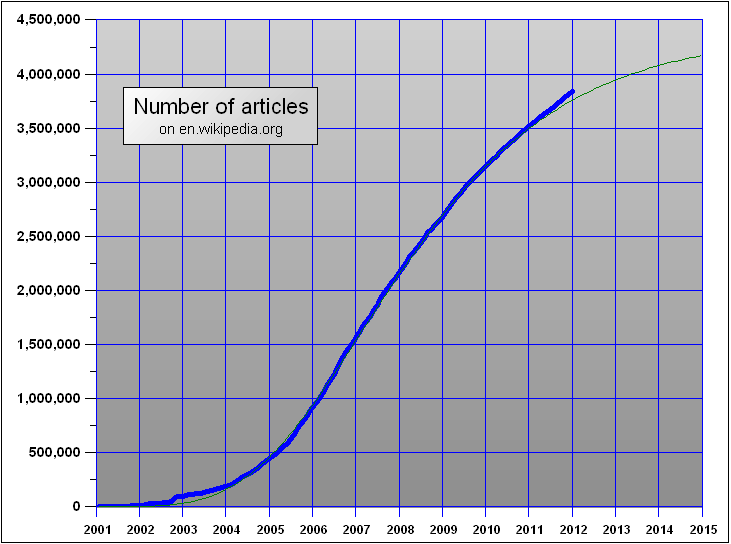
\includegraphics[scale=0.30]{presentation/EnwikipediaGom.PNG}
\end{figure}

\end{itemize}

\end{frame}

%----------------------------------

\begin{frame}{Goals}

\begin{itemize}
 \item Parallization based on Menthor\citep{oai:infoscience.epfl.ch:165111}

\begin{figure}[!htb]
  \centering
  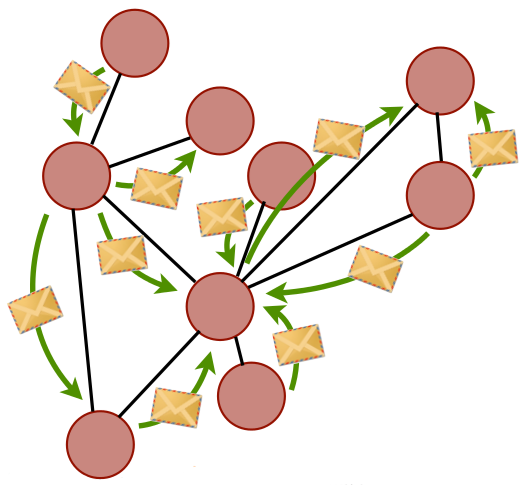
\includegraphics[scale=0.20]{presentation/Menthor.png}
\end{figure}

 \item Implement Maximum Entropy\citep{berger_a1-etal:1996a} and Naive Bayesian\citep{Rennie03}
 \item Benchmark two different parallelization strategies
\end{itemize}

\end{frame}

%----------------------------------

\begin{frame}{Outline}

\begin{itemize}
 \item Motivation
 \item Goals
 \item Outline
 \item Text Categorization
 \item Classification Algorithms
	\begin{itemize}
	\item  Maximum Entropy
	\item  Naive Bayes
	\end{itemize}
 \item Parallelization
	\begin{itemize}
	\item  Maximum Entropy
	\item  Naive Bayes
	\item  Strategy 1: Vertex for every sample
	\item  Strategy 2: Vertex for set of samples
	\end{itemize}
 \item Experimental results
	\begin{itemize}
	\item Data sets
	\item Benchmarks
	\end{itemize}
\end{itemize}

\end{frame}

%----------------------------------

\begin{frame}{Text Categorization}

\begin{figure}[!htb]
  \centering
  
\includegraphics[scale=0.6]{presentation/text_categorization.jpg}
\end{figure}

\begin{itemize}
 \item Determine the category of a document
 \item Predefined categories
 \item Spam filtering - spam or not spam
\end{itemize}

\end{frame}

%----------------------------------

\begin{frame}{Classification Algorithms - Maximum Entropy}

\begin{itemize}
 \item The probability should be as uniform as possible, i.e. have maximum entropy

\begin{equation}
\label{mx:expdistr}
P_{\Lambda}(c|s) = \frac{1}{Z(s)} \sum_{i}\exp(\lambda_i f_i(s,c))
\end{equation}

 \item Improved Iterative Scaling

\begin{itemize}
	\item \textbf{Inputs:} Set $S$ of labeled samples and a set of feature functions $f_i$.
	\item Estimate expected value of $f_i$ on the training samples.
	\item Initialize all the parameters $\lambda_i$'s to be zero.
	\item Iterate until convergence:
	\begin{itemize}
		\item Calculate the expected class labels for each sample with $P_{\Lambda}(c|s)$
		\item For each parameter $\lambda_i$: Find $\delta_i  = \frac{1}{M} \log \frac{\sum_{s \in S} f_i (s|c(s))}{\sum_{s \in S}\sum_{c} P_{\Lambda}(c|s) f_i(s|c) }$, and set $\lambda_i = \lambda_i + \delta_i$
	\end{itemize}		
	\item \textbf{Output:} A classifier that predicts the class label of sample  $s$.
\end{itemize}

\end{itemize}

\end{frame}

%----------------------------------

\begin{frame}{Classification Algorithms - Naive Bayes}

\begin{itemize}
 \item Based on the Bayes's Rule
\[
P(C|S) = \frac{P (S|C) P (C)}{P(S)} = \frac{P (S|C) P (C)}{\sum_{c \in C} P(D|C=c)P(C=c)}
\] 
\item Probability estimation

\[
P(c) = \frac{N_c}{N}
\]

\[
P(s|c) = \prod_{w} P(w|c)^{tf_{w,s}}
\]

\[
P(w|c) = \frac{tf_{w,c}}{|c|}
\]

	\begin{itemize}
	\item $N_c$ - \# of samples that have class $c$
	\item $tf_{w,s}$ - \# of times term $w$ occurs in sample $s$
	\item $tf_{w,c}$ - \# of times term $w$ occurs in class $c$
	\item $|c|$ - total number of terms in class $C$
	\end{itemize}

\end{itemize}

\end{frame}

%----------------------------------

\begin{frame}{Parallelization - Maximum Entropy}

\begin{itemize}
 \item Mixture Weight Method \citep{conf/nips/MannMMSW09}

\begin{figure}[!htb]
  \centering
  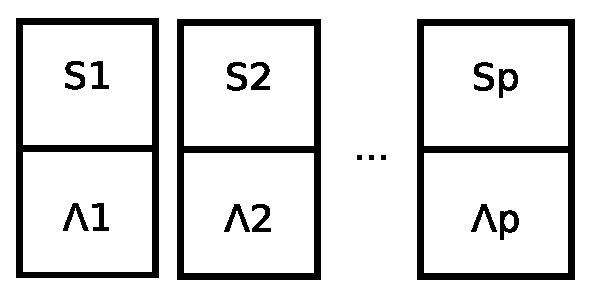
\includegraphics[scale=0.50]{presentation/mixture_weight.eps}
\end{figure}

\[
\Lambda_{\mu} = \sum_{k=1}^{p} \frac{1}{p} \Lambda_{k}
\]

\item Not good for small training sets

\end{itemize}

\end{frame}

%----------------------------------

\begin{frame}{Parallelization - Naive Bayes}

\begin{itemize}

\item Split the training data and then mix

\begin{figure}[!htb]
  \centering
  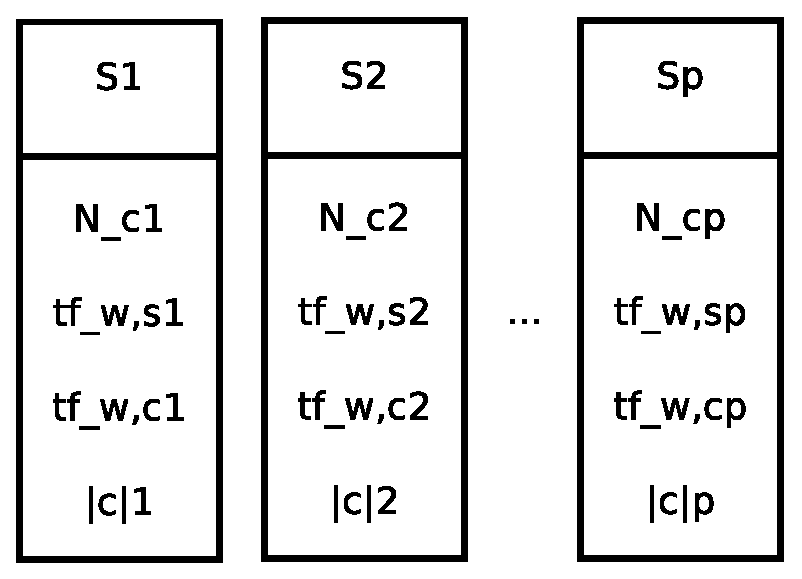
\includegraphics[scale=0.40]{presentation/naive_bayes_split.eps}
\end{figure}

\item No accuracy lose

\end{itemize}

\end{frame}

%----------------------------------

\begin{frame}{Parallelization - Strategy 1: Vertex for every sample}

\begin{itemize}
\item Every sample is a vertex  
\item Master vertex for aggregation
\item $|S| + p(p-1)$ message exchanges 
\item Signification communication overhead
\end{itemize}

\begin{figure}[!htb]
  \centering
  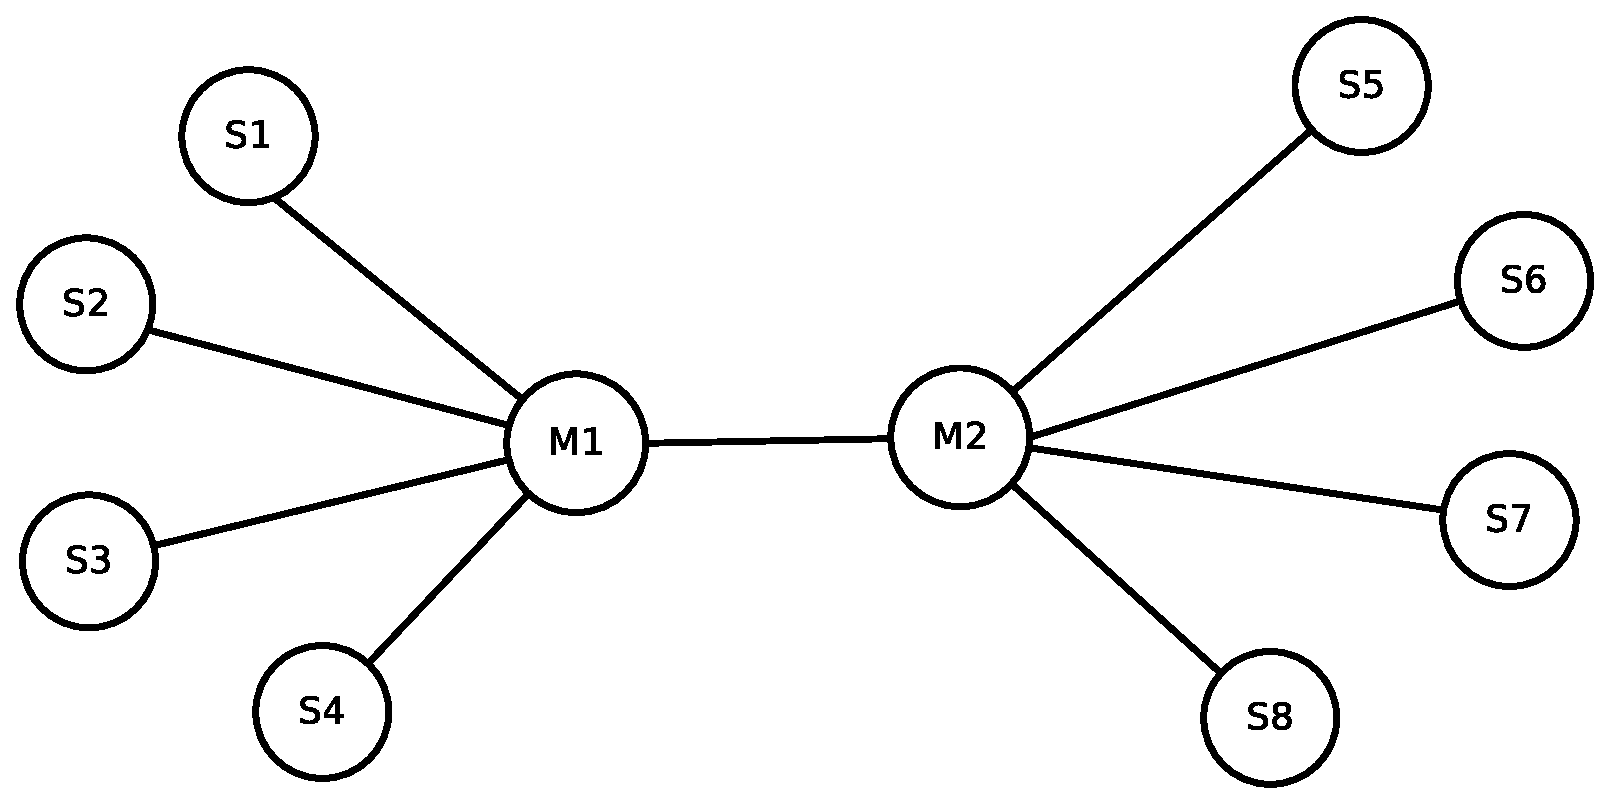
\includegraphics[scale=0.30]{graph1.eps}
  \label{fig:vs:graph1}
\end{figure}

\end{frame}

%----------------------------------

\begin{frame}{Parallelization - Strategy 2: Vertex for set of samples}

\begin{itemize}
\item Vertex for each partition 
\item The vertex has set of samples
\item $p(p-1)$ message exchanges
\item Low communication overhead
\end{itemize}

\begin{figure}[!htb]
  \centering
  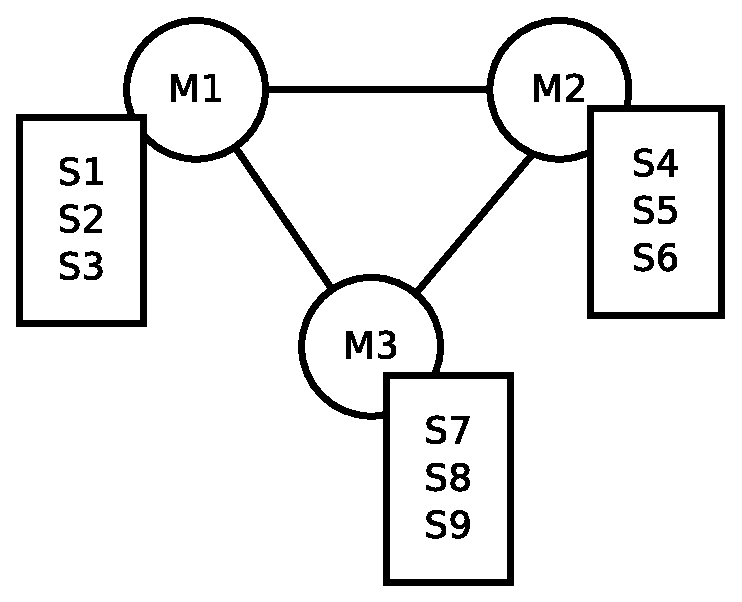
\includegraphics[scale=0.30]{graph2.eps}
  \label{fig:vss:graph2}
\end{figure}

\end{frame}

%----------------------------------

\begin{frame}{Experimental results - Data sets}

\begin{itemize}
\item Movie Reviews\citep{Pang+Lee:04a}

\begin{itemize}
\item 2000 movie reviews: 1000 positive and 1000 negative
\item 100 features
\end{itemize}

\begin{table}[ht]
\centering
\begin{tabular}{ l c }
    \hline\hline
    Algorithm & Accuracy \\ [0.2ex]
    \hline
    Maximum Entropy &  86.33 \\ % 84.92462, 83.91959, 87.9397, 84.92462, 89.94472
    Naive Bayes & 85.62 \\ % 86.43216, 89.447235, 81.407036, 86.43216, 84.42211
    \hline
  \end{tabular}
\label{table:mrprecision}
\end{table}

\end{itemize}

\end{frame}

%----------------------------------

\begin{frame}{Experimental results - Data sets}

\begin{itemize}
\item 20 Newsgroups \footnote{people.csail.mit.edu/jrennie/20Newsgroups}

\begin{itemize}
\item 25000 document
\item 18846 training examples, and 7532 test examples
\item 20 categories
\item 5000 features
\end{itemize}

\begin{table}[ht]
\centering
\begin{tabular}{ l c }
    \hline\hline
    Algorithm & Accuracy \\ [0.2ex]
    \hline
    Maximum Entropy &  57.44 \\
    Naive Bayes & 92.12  \\
    \hline
  \end{tabular}
\label{table:20nprecision}
\end{table}

\end{itemize}

\end{frame}

%----------------------------------

\begin{frame}{Experimental results - Data sets}

\begin{itemize}
\item Wikipedia INEX 2009 collection \citep{conf/btw/SchenkelSK07}

\begin{itemize}
\item Prepared for evaluating information retrieval tasks
\item 2,666,190 articles from Wikipedia; we use a subsets of 40,000 articles
\item 331 categories taken from Dbpedia\footnote{dbpedia.org/About}
\item 10000 features
\end{itemize}

\end{itemize}

\end{frame}

%----------------------------------

\begin{frame}{Experimental results - Benchmark Methodology}

\begin{itemize}

\item 8 cores machine
\item 40 000 articles from wikipedia
\item 5 runs for every core, ignore the first one

\end{itemize}

\end{frame}

%----------------------------------

\begin{frame}{Experimental results - Maximum Entropy Benchmarks}

\begin{itemize}

\item{Vertex for a set of sample}

\begin{itemize}
\item 1.65x times faster for every 2 cores on average
\item 1.86x times between 1 and 2 cores
\item 7.38x times between 1 and 8 cores
\end{itemize}

\begin{figure}[!htb]
  \centering
  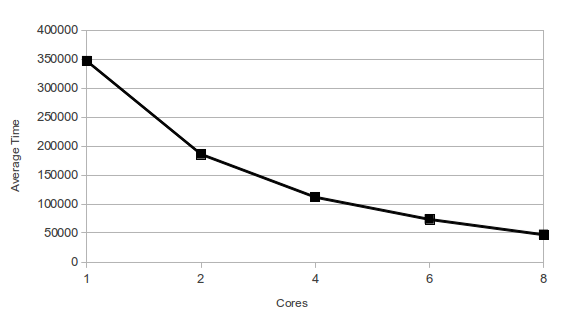
\includegraphics[scale=0.35]{maxent_plot.png}
  \label{fig:maxent_plot}
\end{figure}

\end{itemize}

\end{frame}

%----------------------------------

\begin{frame}{Experimental results - Maximum Entropy Benchmarks}

\begin{itemize}

\item{Vertex for every sample}

\begin{itemize}
\item  5241952 ms  on 8 cores 
\item  111x times slower
\end{itemize}

\item{Sequential}

\begin{itemize}
\item No improvement between 1 and 8 cores
\item Parallel version is 1.40x times faster
\end{itemize}

\begin{table}[!htb]
\centering
\begin{tabular}{ l c }
    \hline\hline
    Cores & Avarage Time \\ [0.2ex]
    \hline
    1 & 67235 \\
    8 & 67140  \\
    \hline
  \end{tabular}
\label{table:maxentres2}
\end{table}

\end{itemize}

\end{frame}

%----------------------------------

\begin{frame}{Experimental results - Naive Bayes Benchmarks}

\begin{itemize}

\item{Vertex for a set of sample}

\begin{itemize}
\item 1.52x times faster for every 2 cores on average
\item 1.79x times between 1 and 2 cores
\item 5.25x times between 1 and 8 cores
\end{itemize}

\begin{figure}[!htb]
  \centering
  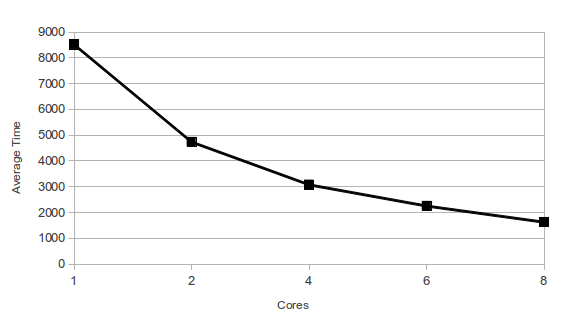
\includegraphics[scale=0.35]{naivebayes_plot.png}
  \label{fig:naive_plot}
\end{figure}

\end{itemize}

\end{frame}

%----------------------------------

\begin{frame}{Experimental results -  Naive Bayes Benchmarks}

\begin{itemize}

\item{Vertex for every sample}

\begin{itemize}
\item  62300.5 ms on 8 cores 
\item  38x times slower
\end{itemize}

\item{Sequential}

\begin{itemize}
\item No improvement between 1 and 8 cores
\item Parallel version is 3.10x times faster
\end{itemize}

\begin{table}[!htb]
\centering
\begin{tabular}{ l c }
    \hline\hline
    Cores & Average Time \\ [0.2ex]
    \hline
    1 & 5224.75 \\
    8 & 5579.75  \\
    \hline
  \end{tabular}
\label{table:naivebayes2}
\end{table}

\end{itemize}

\end{frame}

%----------------------------------

\begin{frame}{Experimental results - Comparison}

\begin{figure}[!htb]
  \centering
  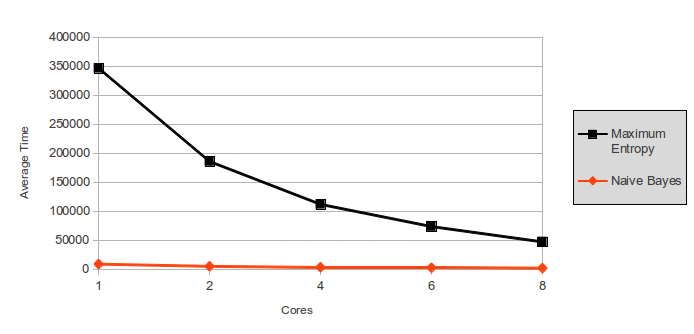
\includegraphics[scale=0.45]{presentation/comparison.png}
\end{figure}

\end{frame}

%----------------------------------

\begin{frame}{Conclusion}
Menthor makes it easy to implement parallel machine learning algorithms without much effort and with excellent scalability.
\end{frame}

%----------------------------------

\begin{frame}{The end}
Questions ?
\end{frame}

\begin{frame}[allowframebreaks]{References}
\bibliographystyle{plainnat}
\bibliography{references}
\end{frame}

\end{document}